\documentclass[a4paper]{article}
\usepackage{tikz}
\usepackage{geometry}
\usepackage{graphicx}
\usepackage{natbib}
\usepackage{amsmath}
\usepackage{amssymb}
\usepackage{amsthm}
\usepackage{paralist}
\usepackage{epstopdf}
\usepackage{tabularx}
\usepackage{longtable}
\usepackage{multirow}
\usepackage{multicol}
\usepackage[hidelinks]{hyperref}
\usepackage{fancyvrb}
\usepackage{algorithm}
\usepackage{algorithmic}
\usepackage{float}
\usepackage{paralist}
%\usepackage[svgname]{xcolor}
\usepackage{enumerate}
\usepackage{array}
\usepackage{times}
\usepackage{url}
\usepackage{fancyhdr}
\usepackage{comment}
\usepackage{environ}
\usepackage{times}
\usepackage{textcomp}
\usepackage{caption}
\usepackage{bbm}


\urlstyle{rm}

\setlength\parindent{0pt} % Removes all indentation from paragraphs
\theoremstyle{definition}
\newtheorem{definition}{Definition}[]
\newtheorem{conjecture}{Conjecture}[]
\newtheorem{example}{Example}[]
\newtheorem{theorem}{Theorem}[]
\newtheorem{lemma}{Lemma}
\newtheorem{proposition}{Proposition}
\newtheorem{corollary}{Corollary}

\floatname{algorithm}{Procedure}
\renewcommand{\algorithmicrequire}{\textbf{Input:}}
\renewcommand{\algorithmicensure}{\textbf{Output:}}
\newcommand{\abs}[1]{\lvert#1\rvert}
\newcommand{\norm}[1]{\lVert#1\rVert}
\newcommand{\RR}{\mathbb{R}}
\newcommand{\CC}{\mathbb{C}}
\newcommand{\Nat}{\mathbb{N}}
\newcommand{\br}[1]{\{#1\}}
\DeclareMathOperator*{\argmin}{arg\,min}
\DeclareMathOperator*{\argmax}{arg\,max}
\renewcommand{\qedsymbol}{$\blacksquare$}

\definecolor{dkgreen}{rgb}{0,0.6,0}
\definecolor{gray}{rgb}{0.5,0.5,0.5}
\definecolor{mauve}{rgb}{0.58,0,0.82}

\newcommand{\Var}{\mathrm{Var}}
\newcommand{\Cov}{\mathrm{Cov}}

\newcommand{\vc}[1]{\boldsymbol{#1}}
\newcommand{\xv}{\vc{x}}
\newcommand{\Sigmav}{\vc{\Sigma}}
\newcommand{\alphav}{\vc{\alpha}}
\newcommand{\muv}{\vc{\mu}}

\newcommand{\red}[1]{\textcolor{red}{#1}}

\def\x{\mathbf x}
\def\y{\mathbf y}
\def\w{\mathbf w}
\def\v{\mathbf v}
\def\E{\mathbb E}
\def\R{\mathbb R}
\def\V{\mathbb V}
\def\ind{\mathbbm 1}

% TO SHOW SOLUTIONS, include following (else comment out):
\newenvironment{soln}{
    \leavevmode\color{blue}\ignorespaces
}{}


\hypersetup{
%    colorlinks,
    linkcolor={red!50!black},
    citecolor={blue!50!black},
    urlcolor={blue!80!black}
}

\geometry{
  top=1in,            % <-- you want to adjust this
  inner=1in,
  outer=1in,
  bottom=1in,
  headheight=3em,       % <-- and this
  headsep=2em,          % <-- and this
  footskip=3em,
}


\pagestyle{fancyplain}
\lhead{\fancyplain{}{Homework 6}}
\rhead{\fancyplain{}{CS 760 Machine Learning}}
\cfoot{\thepage}

\title{\textsc{Homework 6}} % Title

%%% NOTE:  Replace 'NAME HERE' etc., and delete any "\red{}" wrappers (so it won't show up as red)

\author{
\red{$AKASH SHARMA$} \\
\red{$9081731771$}\\
} 

\date{}

\begin{document}

\maketitle 


\textbf{Instructions:} 
Although this is a programming homework, you only need to hand in a pdf answer file.
There is no need to submit the latex source or any code.
You can choose any programming language, as long as you implement the algorithm from scratch. 

Use this latex file as a template to develop your homework.
Submit your homework on time as a single pdf file to Canvas.
Please check Piazza for updates about the homework.

10 points each.

\section{Neural Network Family Portrait}
A fixed feedforward neural network architecture induces a family of functions $\{f_w: X \mapsto Y\}$ with different edge weights $w$.
In this question you will randomly generate members of the family and visualize the function mapping. 
This helps us understand the variety of functions that neural networks can produce. 
For visualization, the input is $x=(x_1, x_2) \in \R^2$ and the output is $y\in\R$.

\begin{enumerate}
\item Implement a single hidden layer with 10 ReLU units.
The $i$th ReLU unit has weights $b_i, w_{i1}, w_{i2}$ and outputs 
$$o_i =\max( b_i + w_{i1} x_1 + w_{i2} x_2, 0).$$
Implement an output layer with a single sigmoid unit.
It has weights $b_o, w_{o1}, \ldots, w_{o,10}$ and outputs
$$y =\sigma( b_o + w_{o1} o_1 + \ldots + w_{o,10} o_{10})$$
where $\sigma()$ is the sigmoid function.
For this question, set \emph{all} $b$ and $w$ to 1.
Show the value of $o_1, \ldots, o_{10}, y$ for three input points, respectively: $x=(1,1), x=(1, -1), x=(-1,-1)$.

\begin{soln}
(1)When x = (1, 1)
\\$o_1$ = 3.0, $o_2$ = 3.0, $o_3$ = 3.0, $o_4$ = 3.0, $o_5$ = 3.0, $o_6$ = 3.0, $o_7$ = 3.0, $o_8$ = 3.0, $o_9$ = 3.0, $o_{10}$ = 3.0, 
\\y = 0.99999999999996558309

(2) When x = (1, -1)
\\$o_1$ = 1.0, $o_2$ = 1.0, $o_3$ = 1.0, $o_4$ = 1.0, $o_5$ = 1.0, $o_6$ = 1.0, $o_7$ = 1.0, $o_8$ = 1.0, $o_9$ = 1.0, $o_{10}$ = 1.0, 
\\y = 0.99998329857815204669

(3) When x = (-1, -1)
\\$o_1$ = 0.0, $o_2$ = 0.0, $o_3$ = 0.0, $o_4$ = 0.0, $o_5$ = 0.0, $o_6$ = 0.0, $o_7$ = 0.0, $o_8$ = 0.0, $o_9$ = 0.0, $o_{10}$ = 0.0, 
\\y = 0.73105857863000489605

\end{soln}



\item Now generate a random network by drawing each and every $b$, $w$ independently from a standard Gaussian $N(0,1)$.
With this random network $f_w$, visualize $y=f_w(x)$ for $x=(x_1,x_2)$ on the 2D grid $x_1 \in [-5,5], x_2 \in [-5, 5]$.
You can do this with a 3D surface plot, a 2D contour plot, or whatever is visually clear and convenient for your programming language.
If you are not familiar with visualization in your language, ask on Piazza.
For example, in Matlab with meshgrid(-5:0.1:5, -5:0.1:5) and surf(X,Y,F) my random network looks like
%\fbox{\includegraphics[width=4in]{1x10ReLu1Sigmoid.pdf}}
We ask you to generate as many random networks as you like, but visualize the first three networks (so they are an unbiased sample), then visualize three more networks that you find interesting among the ones you generate.
That is a total of six plots.
\begin{soln}


The plots with each and every $b$, $w$ generated independently from a standard Gaussian $N(0,1)$ are shown below:

\begin{figure}[h!]
	        \centering
	        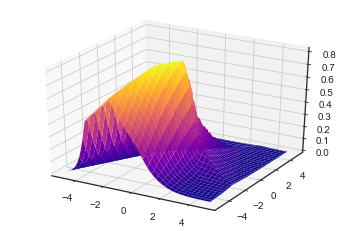
\includegraphics[width=0.6\textwidth]{Q2/Img1.png} 
	        \captionsetup{labelformat=empty}
	        \caption{Plot 1}
	        %\label{fig:Plot of round vs. training set error}



	        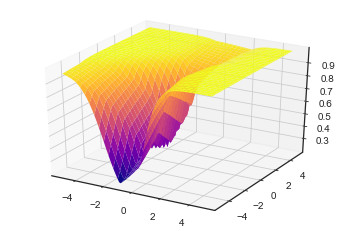
\includegraphics[width=0.6\textwidth]{Q2/Img2.png} 
	        \captionsetup{labelformat=empty}
	        \caption{Plot 2}
	        %\label{fig:Plot of round vs. training set error}


	        \centering
	        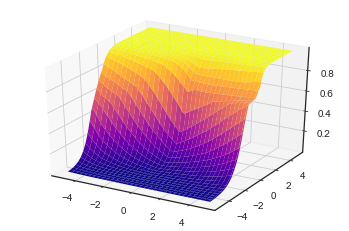
\includegraphics[width=0.6\textwidth]{Q2/Img3.png} 
	        \captionsetup{labelformat=empty}
	        \caption{Plot 3}
	        %\label{fig:Plot of round vs. training set error}
\end{figure}

\begin{figure}[h!]
	        \centering
	        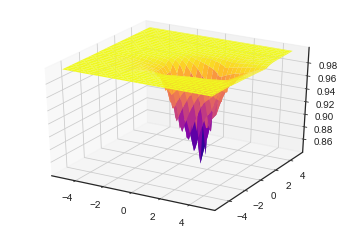
\includegraphics[width=0.6\textwidth]{Q2/Img4.png} 
	        \captionsetup{labelformat=empty}
	        \caption{Plot 4}
	        %\label{fig:Plot of round vs. training set error}


	        \centering
	        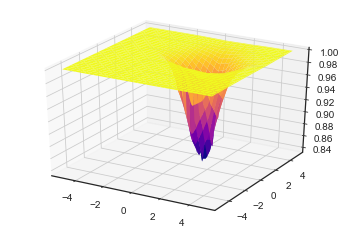
\includegraphics[width=0.6\textwidth]{Q2/Img5.png} 
	        \captionsetup{labelformat=empty}
	        \caption{Plot 5}
	        %\label{fig:Plot of round vs. training set error}


	        \centering
	        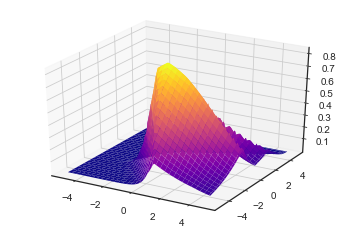
\includegraphics[width=0.6\textwidth]{Q2/Img6.png} 
	        \captionsetup{labelformat=empty}
	        \caption{Plot 6}
	        %\label{fig:Plot of round vs. training set error}
\end{figure}


\end{soln}


\clearpage

\item Repeat question 1 but with 5 hidden layers each with 2 ReLU units (the first hidden layer produces output $o_1, o_2$, and so on).  Same single sigmoid output unit.  This is a deeper network.
For this question, set \emph{all} $b$ and $w$ to 1.
Show the value of $o_1, \ldots, o_{10}, y$ for three input points, respectively: $x=(1,1), x=(1, -1), x=(-1,-1)$.

\begin{soln}
(1) When x = (1, 1)
\\$o_1$ = 3.0, $o_2$ = 3.0, $o_3$ = 7.0, $o_4$ = 7.0, $o_5$ = 15.0, $o_6$ = 15.0, $o_7$ = 31.0, $o_8$ = 31.0, $o_9$ = 63.0, $o_{10}$ = 63.0, 
\\y = 1.0

(2) When x = (1, -1)
\\$o_1$ = 1.0, $o_2$ = 1.0, $o_3$ = 3.0, $o_4$ = 3.0, $o_5$ = 7.0, $o_6$ = 7.0, $o_7$ = 15.0, $o_8$ = 15.0, $o_9$ = 31.0, $o_{10}$ = 31.0, 
\\y = 1.0

(3) When x = (-1, -1)
\\$o_1$ = 0.0, $o_2$ = 0.0, $o_3$ = 1.0, $o_4$ = 1.0, $o_5$ = 3.0, $o_6$ = 3.0, $o_7$ = 7.0, $o_8$ = 7.0, $o_9$ = 15.0, $o_{10}$ = 15.0, 
\\y = 0.99999999999996558308

\end{soln}


\item Repeat question 2 but with the 5-hidden-layer network.
For example, one of my random network is visualized as
%\fbox{\includegraphics[width=4in]{5x2ReLu1Sigmoid.pdf}}
Produce those six plots.

\begin{soln}

\begin{figure}[h!]
	        \centering
	        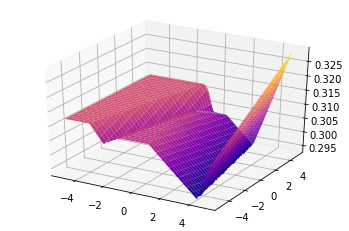
\includegraphics[width=0.6\textwidth]{Q4/Img1.png} 
	        \captionsetup{labelformat=empty}
	        \caption{Plot 1}
	        %\label{fig:Plot of round vs. training set error}
\end{figure}

\begin{figure}[h!]
	        \centering
	        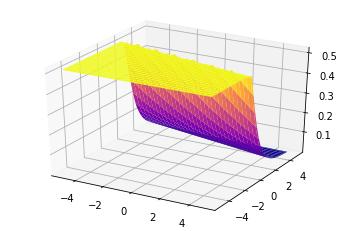
\includegraphics[width=0.6\textwidth]{Q4/Img2.png} 
	        \captionsetup{labelformat=empty}
	        \caption{Plot 2}
	        %\label{fig:Plot of round vs. training set error}
\end{figure}


\begin{figure}[h!]
	        \centering
	        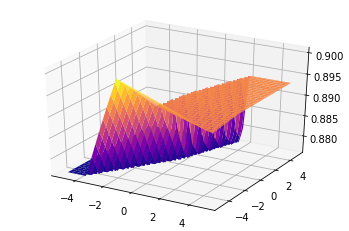
\includegraphics[width=0.6\textwidth]{Q4/Img3.png} 
	        \captionsetup{labelformat=empty}
	        \caption{Plot 3}
	        %\label{fig:Plot of round vs. training set error}
\end{figure}

\begin{figure}[h!]
	        \centering
	        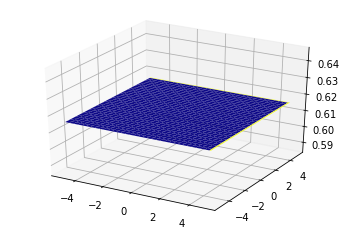
\includegraphics[width=0.6\textwidth]{Q4/Img4.png} 
	        \captionsetup{labelformat=empty}
	        \caption{Plot 4}
	        %\label{fig:Plot of round vs. training set error}
\end{figure}

\begin{figure}[h!]
	        \centering
	        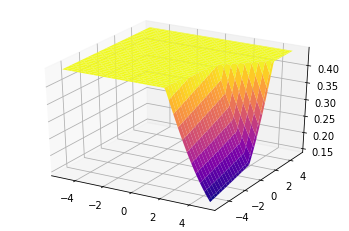
\includegraphics[width=0.6\textwidth]{Q4/Img5.png} 
	        \captionsetup{labelformat=empty}
	        \caption{Plot 5}
	        %\label{fig:Plot of round vs. training set error}
\end{figure}

\begin{figure}[h!]
	        \centering
	        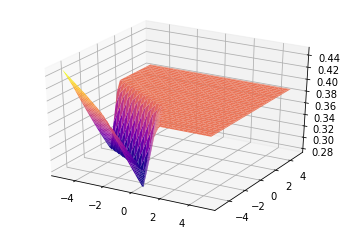
\includegraphics[width=0.6\textwidth]{Q4/Img6.png} 
	        \captionsetup{labelformat=empty}
	        \caption{Plot 6}
	        %\label{fig:Plot of round vs. training set error}
\end{figure}


\end{soln}


\end{enumerate}

\clearpage

\section{Back Propagation}

We will build a neural network to perform binary classification.
Each input item has two real-valued features $x=(x_1, x_2)$, and the class label $y$ is either 0 or 1.
Our neural network has a very simple structure: 

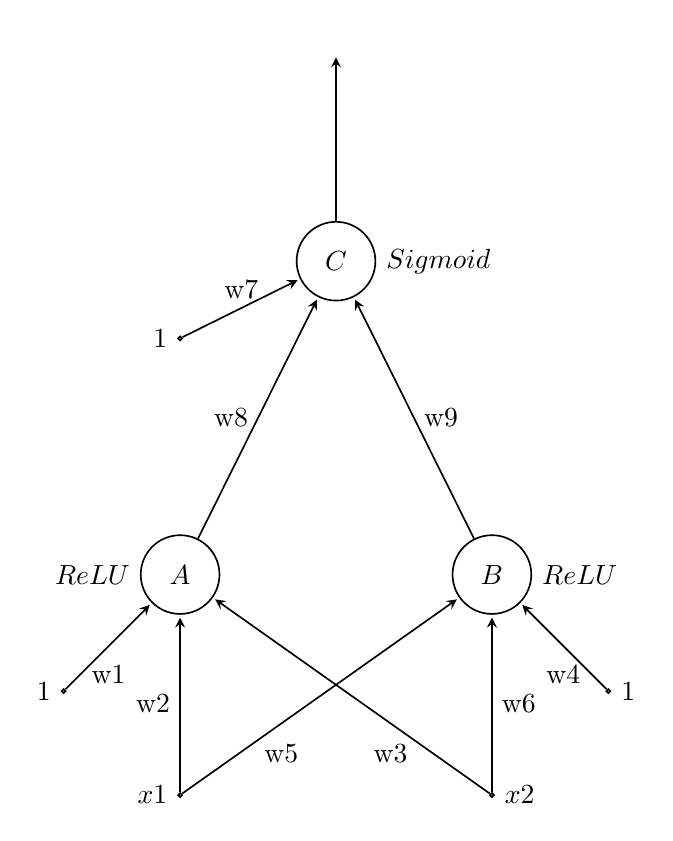
\begin{tikzpicture}[->,>=stealth,shorten >=1pt,auto,node distance=2.8cm,
                    semithick]
  \tikzstyle{state}=[circle,draw=black,text=black,minimum size=1cm]
  \tikzstyle{point}=[circle,draw=black,text=black,inner sep=0pt, minimum size=0.5mm]

  \node[state]         (A) [label=left:$ReLU$] {$A$};
  \node[state]         (C) [above right of=A, yshift=2cm, label=right:$Sigmoid$] {$C$};
  \node[state]         (B) [below right of=C, yshift=-2cm, label=right:$ReLU$] {$B$};
  \node[point]         (X1) [below of=A,label=left:$x1$] {};
  \node[point]         (X2) [below of=B,label=right:$x2$] {};
  \node[point]         (Y1) [below left of=A, xshift=0.5cm, yshift=0.5cm, label=left:$1$] {};
  \node[point]         (Y2) [below right of=B, xshift=-0.5cm, yshift=0.5cm, label=right:$1$] {};
  \node[point]         (Y3) [below left of=C, yshift=1cm, label=left:$1$] {};
  \node[circle]        (Z) [above of=C] {};




  \path (A) edge              node [left] {w8} (C)
        (B) edge              node [right] {w9} (C)
        (C) edge              node {} (Z)
        (X1) edge             node {w2} (A)
             edge             node [below, xshift=-0.5cm, yshift=-0.5cm] {w5} (B)
        (X2) edge             node [below, xshift=0.5cm, yshift=-0.5cm] {w3} (A)
             edge             node [right] {w6} (B)
        (Y1) edge             node [above, yshift=-6mm] {w1} (A)
        (Y2) edge             node [above, yshift=-6mm] {w4} (B)
        (Y3) edge             node [above] {w7} (C);
\end{tikzpicture}

There is one hidden layer with two hidden units A, B, and one output layer with a single output unit C.
The input layer is fully connected to the hidden layer, and the hidden layer is fully connected to the output layer.
Each unit also has a constant bias 1 input with the corresponding weight. 
Units A are B are ReLU, namely 
$$f_A(z)=f_B(z)=\max(z, 0).$$
Unit C is a sigmoid:
$$f_C(z)=\sigma(z)=\frac{1}{1+e^{-z}}.$$

Implement the following steps. 
We provide a few examples for you to debug your code.

\begin{enumerate}
\item
This neural network is fully defined by the nine weights $w_1, \ldots, w_9$.
The first question first focuses on predictions \emph{given} fixed weights.

Remark: we will use both single index and double index to refer to a weight.
Single index corresponds to the figure above.
Double index, on the other hand, is used to describe the algorithm and denotes the ``from $\rightarrow$ to'' nodes that the edge is connecting.
For example, $w_8$ is the same as $w_{A,C}$, $w_2$ is the same as $w_{x_1, A}$, and $w_1$ is the same as $w_{1,A}$ where we used ``1'' to denote the constant bias input of one.
These should be clear from the context.

Recall in a neural network for any unit $j$, it first collects input from lower units:
$$u_j = \sum_{i: i\rightarrow j} w_{ij} v_i$$
where $v_i$ is the output of lower unit $i$. Specifically, if $i$ is an input unit then $v_i=x_i$; if $i$ is the bias then $v_i=1$.
The unit $j$ then passes $u_j$ through its nonlinear function $f_j()$ to produce its output $v_j$:
$$v_j = f_j(u_j).$$

Given weights $w_1, \ldots, w_9$ and input $x_1$, $x_2$,
print $u_A, v_A, u_B, v_B, u_C, v_C$ on the same line separated by space. 
For example,
\begin{verbatim}
(weights) 0.1 0.2 0.3 0.4 0.5 0.6 0.7 0.8 0.9 (input) 1 -1
0.00000 0.00000 0.30000 0.30000 0.97000 0.72512 

(weights) 1 0.9 0.8 0.7 0.6 0.5 0.4 0.3 0.2 (input) -0.2 1.7
2.18000 2.18000 1.43000 1.43000 1.34000 0.79249 

(weights) 4 3 2 1 0 -1 -2 -3 -4 (input) -4 1
-6.00000 0.00000 0.00000 0.00000 -2.00000 0.11920 
\end{verbatim}

Now compute $u_A, v_A, u_B, v_B, u_C, v_C$ for weights 0.1 -0.2 0.3 -0.4 0.5 -0.6 0.7 -0.8 0.9 and input 1 -1.

\begin{soln}

\begin{verbatim}
(weights) 0.1  -0.2  0.3  -0.4  0.5  -0.6  0.7  -0.8  0.9 (input) 1 -1
-0.40000 0.00000 0.70000 0.70000 1.33000 0.79084
\end{verbatim}

\end{soln}


\item
Given a training item $x=(x_1, x_2)$ and its label $y$, the squared error made by the neural network on the item is defined as
$$E = \frac{1}{2}(v_C - y)^2.$$
The partial derivative with respect to the output layer variable $v_C$ is 
$$\frac{\partial E}{\partial v_C} = v_C - y.$$
The partial derivative with respect to the intermediate variable $u_C$ is 
$$\frac{\partial E}{\partial u_C} = \frac{\partial E}{\partial v_C} f_C'(u_C).$$
Recall $f_C'(u_C) = \sigma'(u_C) = \sigma(u_C)(1-\sigma(u_C)) = v_C (1-v_C)$.

Print $E$, $\frac{\partial E}{\partial v_C}$, and $\frac{\partial E}{\partial u_C}$. 
For example,
\begin{verbatim}
(weights) 0.1 0.2 0.3 0.4 0.5 0.6 0.7 0.8 0.9 (input) 1 -1 (y) 1
0.03778 -0.27488 -0.05479

(weights) 1 0.9 0.8 0.7 0.6 0.5 0.4 0.3 0.2 (input) -0.2 1.7 (y) 0
0.31402 0.79249 0.13032

(weights) 4 3 2 1 0 -1 -2 -3 -4 (input) -4 1 (y) 0
0.00710 0.11920 0.01252
\end{verbatim}

Now compute $E$, $\frac{\partial E}{\partial v_C}$, and $\frac{\partial E}{\partial u_C}$ for weights 0.1 -0.2 0.3 -0.4 0.5 -0.6 0.7 -0.8 0.9, input 1 -1, and label $y=1$.

\begin{soln}

\begin{verbatim}
(weights) 0.1 -0.2 0.3 -0.4 0.5 -0.6 0.7 -0.8 0.9 (input) 1 -1 (y) 1
0.02187 -0.20916 -0.03460
\end{verbatim}

\end{soln}

\item 
The partial derivative with respect to hidden layer variable $v_j$ is
$$\frac{\partial E}{\partial v_j} = \sum_{k: j\rightarrow k} w_{jk} \frac{\partial E}{\partial u_k}.$$
And 
$$\frac{\partial E}{\partial u_j} = \frac{\partial E}{\partial v_j} \frac{\partial v_j}{\partial u_j}.$$
Recall our hidden layer units are ReLU, for which
$$\frac{\partial v_j}{\partial u_j}=\frac{\partial \max(u_j, 0)}{\partial u_j}=\left\{
\begin{array}{ll}
1, & u_j \ge 0 \\
0, & u_j < 0 
\end{array}
\right.$$
Note we define the derivative to be 1 when $u_j=0$ (look up subderivative to learn more).

Print $\frac{\partial E}{\partial v_A}$, $\frac{\partial E}{\partial u_A}$, $\frac{\partial E}{\partial v_B}$, and $\frac{\partial E}{\partial u_B}$.
For example
\begin{verbatim}
(weights) 0.1 0.2 0.3 0.4 0.5 0.6 0.7 0.8 0.9 (input) 1 -1 (y) 1
-0.04383 -0.04383 -0.04931 -0.04931

(weights) 1 0.9 0.8 0.7 0.6 0.5 0.4 0.3 0.2 (input) -0.2 1.7 (y) 0
0.03910 0.03910 0.02606 0.02606

(weights) 4 3 2 1 0 -1 -2 -3 -4 (input) -4 1 (y) 0
-0.03755 0.00000 -0.05006 -0.05006
\end{verbatim}
Now print $\frac{\partial E}{\partial v_A}$, $\frac{\partial E}{\partial u_A}$, $\frac{\partial E}{\partial v_B}$, and $\frac{\partial E}{\partial u_B}$ for weights 0.1 -0.2 0.3 -0.4 0.5 -0.6 0.7 -0.8 0.9, input 1 -1, and label $y=1$.

\begin{soln}

\begin{verbatim}
(weights) 0.1 -0.2 0.3 -0.4 0.5 -0.6 0.7 -0.8 0.9 (input) 1 -1 (y) 1
0.02768 0.00000 -0.03114 -0.03114
\end{verbatim}
\end{soln}


\item
Now we can compute the partial derivative with respect to the edge weights:
$$\frac{\partial E}{\partial w_{ij}} = v_i \frac{\partial E}{\partial u_j}.$$
Print $\frac{\partial E}{\partial w_1}, \ldots \frac{\partial E}{\partial w_9}$. 
For example,
\begin{verbatim}
(weights) 0.1 0.2 0.3 0.4 0.5 0.6 0.7 0.8 0.9 (input) 1 -1 (y) 1
-0.04383 -0.04383 0.04383 -0.04931 -0.04931 0.04931 -0.05479 0.00000 -0.01644

(weights) 1 0.9 0.8 0.7 0.6 0.5 0.4 0.3 0.2 (input) -0.2 1.7 (y) 0
0.03910 -0.00782 0.06647 0.02606 -0.00521 0.04431 0.13032 0.28411 0.18636

(weights) 4 3 2 1 0 -1 -2 -3 -4 (input) -4 1 (y) 0
0.00000 0.00000 0.00000 -0.05006 0.20025 -0.05006 0.01252 0.00000 0.00000
\end{verbatim}
Now print $\frac{\partial E}{\partial w_1}, \ldots \frac{\partial E}{\partial w_9}$
for weights 0.1 -0.2 0.3 -0.4 0.5 -0.6 0.7 -0.8 0.9, input 1 -1, and label $y=1$.

\begin{soln}

\begin{verbatim}
(weights) 0.1 -0.2 0.3 -0.4 0.5 -0.6 0.7 -0.8 0.9 (input) 1 -1 (y) 1
0.00000 0.00000 0.00000 -0.03114 -0.03114 0.03114 -0.03460 0.00000 -0.02422
\end{verbatim}
\end{soln}



\item
Now we perform one step of stochastic gradient descent.  With step size $\eta$, we update the weights:
$$w_i = w_i - \eta \frac{\partial E}{\partial w_i}, \;\; i=1\ldots 9.$$
For weights $w_1, \ldots, w_9$, input $x_1$, $x_2$, label $y$, step size $\eta$,
print four lines:
\begin{enumerate}
\item the old $w_1 \ldots w_9$
\item the error $E$ under the old $w$
\item the updated $w_1 \ldots w_9$
\item the error $E$ after the update
\end{enumerate}
For example,
\begin{verbatim}
(weights) 0.1 0.2 0.3 0.4 0.5 0.6 0.7 0.8 0.9 (x) 1 -1 (y) 1 (eta) 0.1
0.10000 0.20000 0.30000 0.40000 0.50000 0.60000 0.70000 0.80000 0.90000
0.03778
0.10438 0.20438 0.29562 0.40493 0.50493 0.59507 0.70548 0.80000 0.90164
0.03617

(weights) 1 0.9 0.8 0.7 0.6 0.5 0.4 0.3 0.2 (x) -0.2 1.7 (y) 0 (eta) 0.1
1.00000 0.90000 0.80000 0.70000 0.60000 0.50000 0.40000 0.30000 0.20000
0.31402
0.99609 0.90078 0.79335 0.69739 0.60052 0.49557 0.38697 0.27159 0.18136
0.29972

(weights) 4 3 2 1 0 -1 -2 -3 -4 (x) -4 1 (y) 0 (eta) 0.1
4.00000 3.00000 2.00000 1.00000 0.00000 -1.00000 -2.00000 -3.00000 -4.00000
0.00710
4.00000 3.00000 2.00000 1.00501 -0.02002 -0.99499 -2.00125 -3.00000 -4.00000
0.00371
\end{verbatim}
Print these for weights 0.1 -0.2 0.3 -0.4 0.5 -0.6 0.7 -0.8 0.9, input $x$ 1 -1, label $y$ 1, step size $\eta$ 0.1.

\begin{soln}

\begin{verbatim}
(weights) 0.1 -0.2 0.3 -0.4 0.5 -0.6 0.7 -0.8 0.9, (x) 1 -1 (y) 1 (eta) 0.1
0.10000 -0.20000 0.30000 -0.40000 0.50000 -0.60000 0.70000 -0.80000 0.90000
0.02187
0.10000 -0.20000 0.30000 -0.39689 0.50311 -0.60311 0.70346 -0.80000 0.90242
0.02141
\end{verbatim}
\end{soln}



%------
\item
We provide a training data set data.txt where each row is a labeled item $x_1, x_2, y$.
Starting from initial weights 0.1 -0.2 0.3 -0.4 0.5 -0.6 0.7 -0.8 0.9, with step size $\eta$ 0.1,
run SGD for 10000 rounds.  This means in each round you have to select a training item uniformly randomly from data.txt.
After every 100 rounds, compute the training set error $\sum_i E_i$ where $E_i$ is the $i$-th training item.
Use these to make a plot of round vs. training set error.

\begin{figure}[h!]
	        \centering
	        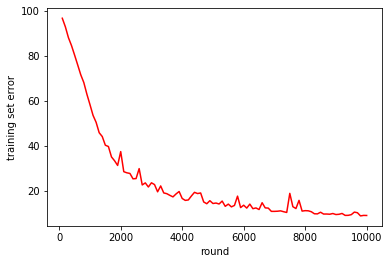
\includegraphics[width=0.6\textwidth]{Q6.png} 
	        \captionsetup{labelformat=empty}
	        \caption{round vs. training set error}
	        \label{fig: round vs. training set error}
\end{figure}


\end{enumerate}



\end{document}
\bibliographystyle{apalike}
\end{document}
